%\documentclass{article}
%\usepackage{graphicx,subfigure}
%\begin{document}

\begin{figure}[h]
  \centering
   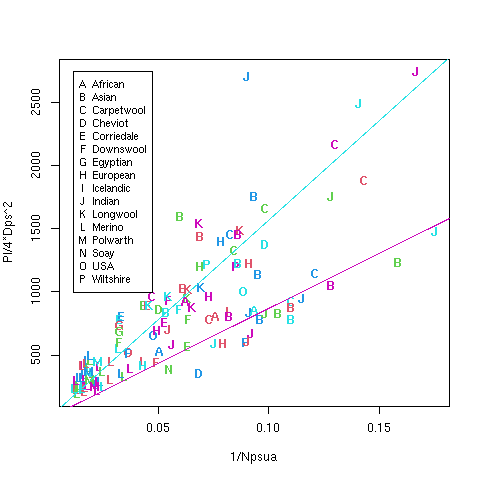
\includegraphics[width=0.9\textwidth]{cartercsax1ovn2reg.png}
  \caption{Plot of breed means for reciprocal of follicle density and fibre cross sectional area from Carter(1968)~\cite{cart:68}. The blue line is a linear regression fitted with a slope of $15689$ and no intercept. The red line is a linear regression fitted with a slope of 8689 and no intercept.}
  \label{fig:carter1ovnxc2reg}
\end{figure}

%\end{document}

